In this system the ds-server simulates job submissions and job executions by servers, whilst the client handles the job scheduling logic. First ds-server needs to open a socket for the client to connect to (defaulting to port 50000), and then the client must connect and authenticate before any scheduling of jobs can begin.\\
\vspace{.2cm}
The flow of communication between the two whilst using LRR is outlined in the flowchart below.
\begin{center}
    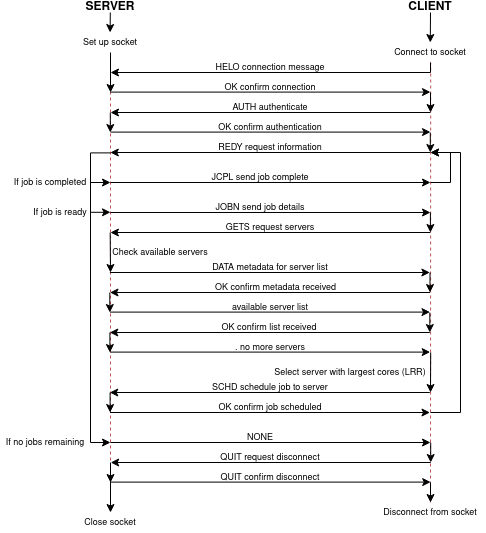
\includegraphics[scale=0.7]{Communication Flowchart.png}
\end{center}

